%\documentclass{ExcelAtFIT}
%\documentclass[czech]{ExcelAtFIT} % when writing in CZECH
\documentclass[slovak]{ExcelAtFIT} % when writing in SLOVAK
\usepackage[binary-units=true,range-units=single]{siunitx}
\sisetup{range-phrase=--}

%--------------------------------------------------------
%--------------------------------------------------------
%	REVIEW vs. FINAL VERSION
%--------------------------------------------------------

%   LEAVE this line commented out for the REVIEW VERSIONS
%   UNCOMMENT this line to get the FINAL VERSION
\ExcelFinalCopy


%--------------------------------------------------------
%--------------------------------------------------------
%	PDF CUSTOMIZATION
%--------------------------------------------------------

\hypersetup{
	pdftitle={Podštruktúrne vyhľadávanie v~databázach chemických látok},
	pdfauthor={Ivan Ševčík},
	pdfkeywords={databáza, vyhľadávanie, grafový izomorfizmus}
}

%--------------------------------------------------------
%--------------------------------------------------------
%	ARTICLE INFORMATION
%--------------------------------------------------------

\ExcelYear{2018}

\PaperTitle{Podštruktúrne vyhľadávanie v~databázach chemických látok}

\Authors{Ivan Ševčík*}
\affiliation{*%
  \href{mailto:xsevci50@stud.fit.vutbr.cz}{xsevci50@stud.fit.vutbr.cz},
  \textit{Faculty of Information Technology, Brno University of Technology}}

\Keywords{Databáza --- Vyhľadávanie vzorov --- Grafový izomorfizmus}

%TODO: Video
%\Supplementary{\href{http://youtu.be/S3msCdn3fNM}{Demonštračné Video} --- \href{https://github.com/BetaRavener/Excel-Substruct}{Dodatočné zdroje}}

\Supplementary{\href{https://github.com/BetaRavener/Excel-Substruct}{Dodatočné zdroje}}


%--------------------------------------------------------
%--------------------------------------------------------
%	ABSTRACT and TEASER
%--------------------------------------------------------

\Abstract{
% What is the problem? What is the topic?, the aim of this paper?
V~tomto článku je predstavený spôsob, pomocou ktorého je možné vyhľadávať zadaný vzor ako podštruktúru v~databázach chemických látok obsahujúcich desiatky miliónov záznamov. Jedná sa o~výpočetne náročný problém, ktorý je potrebné riešiť na niekoľkých úrovniach.	
% How is the problem solved, the aim achieved (methodology)?
Metóda prezentovaná v~tomto článku využíva kombináciu topologických indexov, tzv. molekulárnych odtlačkov, a rýchleho algoritmu pre hľadanie izomorfného podgrafu.
% What are the specific results? How well is the problem solved?
Práca porovnáva niekoľko algoritmov, ako aj spôsobov uloženia molekúl v~systéme. Najlepším riešením sa ukázalo byť použitie algoritmu zvaného RI v~kombinácii s~uložením serializovaných dát do databázy MongoDB. Riešenie umožňuje užívateľom vyhľadávať v~databázach v~reálnom čase, do niekoľkých sekúnd.
% So what? How useful is this to Science and to the reader?
Cieľom tohto článku je oboznámiť čitateľa s~problematikou vyhľadávania v~chemických databázach a ako je možné vytvoriť takýto systém pre vyhľadávanie s~ohľadom na súčasný výskum. Výsledky a myšlienky práce by mohli byť využité v~príbuzných oblastiach vyžadujúcich vyhľadávanie vzorov v~databázach, ako je napríklad počítačové videnie.
}

%TODO:!!! Obrazky
\Teaser{
	\TeaserImage{images/dopamine-teaser.pdf}
	\TeaserImage{images/spacer-teaser.pdf}
	\TeaserImage{images/me-ethanol-teaser.pdf}
}



%--------------------------------------------------------
%--------------------------------------------------------
%--------------------------------------------------------
%--------------------------------------------------------
\begin{document}

\startdocument


%--------------------------------------------------------
%--------------------------------------------------------
%	ARTICLE CONTENTS
%--------------------------------------------------------

%--------------------------------------------------------
%--------------------------------------------------------
%--------------------------------------------------------
%--------------------------------------------------------
\section{Úvod}
%\textbf{[Motivácia]} %What is the raison d'\^{e}tre of your project? Why should anyone care? No general meaningless claims. Make bulletproof arguments for the importance of your work.
Práca sa zaoberá popisom systému, ktorý umožňuje vyhľadávať vzory ako podštruktúry v~databázach chemických látok v~prijateľnom čase. Podštruktúrne vy\-hľa\-dá\-va\-nie má široké uplatnenie. Pomáha nájsť biologicky aktívne alebo toxické látky, urýchľuje výskum nových liečiv a umožňuje identifikovať látky s~chemicky podobnými vlastnosťami. Táto úloha je pomerne dobre preskúmaná a je známy obecný prístup k~jej riešeniu. Pri implementácii je však potrebné zvoliť konkrétne metódy a algoritmy tak, aby sa dosiahlo čo najlepších výsledkov. Súčasťou práce je preto okrem predstavenia návrhu samotného systému umožňujúceho podštruktúrne vy\-hľa\-dá\-va\-nie aj vyhodnotenie a porovnanie dostupných metód s~ohľadom na súčasný stav výskumu.

%\textbf{[Definícia problému]} %What exactly are you solving? What is the core and what is a bonus? What parameters should a proper solution of the problem have? Define the problem precisely and state how its solution should be evaluated.
Vyhľadanie vzoru v~chemickej štruktúre je náročná operácia a problém tiež predstavuje neustále narastajúca veľkosť databáz. Chemické štruktúry sú naj\-čas\-tej\-šie reprezentované formou neorientovaného grafu a vyhľadanie vzoru odpovedá nájdeniu izomorfného podgrafu. Jedná sa o~NP-úplný problém. Výsledkom vyhľadávania je množina všetkých látok uložených v~databáze, ktoré obsahujú zadaný vzor ako podgraf. Pretože je táto operácia často súčasťou rôznych vý\-poč\-tov a predikcií, je nutné aby bola dokončená v~čo najkratšom čase. V~databáze obsahujúcej sto miliónov záznamov by jeden takýto dotaz nemal trvať dlhšie ako niekoľko sekúnd. K~tomu je nutné nájsť nielen rýchly algoritmus, ale aj vhodný topologický index, ktorý umožní predvýber kandidátov, a taktiež optimalizovať spôsob uloženia a načítania molekulárnych dát.

%\textbf{[Existujúce riešenia]} %Discuss existing solutions, be fair in identifying their strengths and weaknesses. Cite important works from the field of your topic. Try to define well what is the \textit{state of the art}. You can include a Section 2 titled ``Background'' or ``Previous Works'' and have the details there and make this paragraph short. Or, you can enlarge this paragraph to a whole page. In many scientific papers, \emph{this} is the most valuable part if it is written properly.
Existuje niekoľko online chemických databáz, kto\-ré podporujú podštruktúrne vyhľadávanie. Medzi jednu z~najväčších patrí databáza PubChem\footnote{\url{https://pubchem.ncbi.nlm.nih.gov/}}. Jedná sa o~uzavreté systémy, ktoré poskytujú požadovanú funkcionalitu, ale sú naviazané na konkrétnu databázu a ich implementácia nie je verejne dostupná. Hlavnou ne\-vý\-ho\-dou sú obmedzenia na využívanie týchto databáz. Napríklad spomínaná databáza PubChem má obmedzenie na svoje REST API na maximálne päť požiadavkov za sekundu, 400 za minútu, a spoločný výpočetný čas operácií nesmie presiahnuť 300 sekúnd za minútu, čo môže nastať pri paralelnom behu po\-žia\-dav\-kov \cite{pubchem_limits}. 

Okrem online sú dôležité aj offline databázy, ktoré sú zdieľané napríklad vo forme súboru. Jedná sa pre\-va\-žne o~súkromné databázy uložené zväčša vo~formáte SDF. K~týmto databázam neexistuje odpovedajúci vy\-hľa\-dá\-va\-cí nástroj. Riešením môže byť použitie jednej z~chemoinformatických knižníc, pomocou ktorých je možné takýto nástroj vytvoriť. Populárna knižnica, od ktorej mnohé ďalšie preberajú koncepty alebo implementáciu, je knižnica RDKit\footnote{\url{http://www.rdkit.org/}}. Zatiaľ čo vytvorenie takéhoto ná\-stro\-ja pre osobné použitie je vďaka knižnici pomerne jednoduché, problém nastáva, ak je potrebné systém pri\-spô\-so\-biť pre konkrétne potreby alebo výrazne šká\-lo\-vať. Napriek tomu predstavuje RDKit vhodnú východiskovú pozíciu. Okrem samotného podštruktúrneho vy\-hľa\-dá\-va\-nia, ktoré je založené na algoritme VF2, poskytuje knižnica taktiež zásuvný modul pre PostgreSQL databázu, ktorá slúži pre uloženie štruktúrnych dát a ďalších informácií o~látkach. Tento modul sprístupňuje vy\-hľa\-dá\-va\-nie na vysokej abstraktnej úrovni pomocou SQL dotazov a samotné vyhľadanie potom prebieha priamo v~procese databázového servera. To ale taktiež znamená, že pri veľkom počte dotazov hrozí preťaženie tohto jedného servera.

%\textbf{[Naše riešenie]}  %Make a quick outline of your approach -- pitch your solution.  The solution will be described in detail later, but give the reader a very quick overview now.
V~tomto článku je predstavené modulárne riešenie, v~ktorom je každá časť systému zodpovedná za špe\-ci\-fi\-ckú úlohu, čo dáva možnosť jednoduchšie škálovať podľa konkrétnej potreby. Tento prístup tiež umožňuje systém oveľa lepšie optimalizovať a zvoliť nástroje, ktoré sú pre daný problém najvhodnejšie. Samotné vyhľadávanie používa rovnaký topologický index ako knižnica RDKit. Pre nájdenie izomorfného podgrafu je však použitý algoritmus RI, ktorý je v~porovnaní s~algoritmom VF2 schopný nájsť riešenie až v~trojnásobne kratšom čase. 

% \textbf{[Dosiahnuté výsledky]} %Sell your solution. Pinpoint your achievements. Be fair and objective.
Výsledkom práce je demonštrácia systému, ktorý umožňuje užívateľom zakresliť požadovaný vzor a vyhľadať ho v~databáze. Dôležitou súčasťou je množina meraní, ktoré umožňujú zodpovedať otázky ohľadom voľby algoritmov a technológií. 

\section{Podštruktúrne vyhľadávanie}
Ako bolo spomenuté v~úvode, chemické štruktúry zvyknú byť reprezentované formou dvojrozmerného neorientovaného grafu, kde vrcholy predstavujú atómy a hrany väzby medzi atómami. Bežnú definíciu grafu je nutné navyše rozšíriť tak, aby každý vrchol a hrana mohli niesť množinu atribútov a hodnôt, ktoré popisujú ich vlastnosti. Atómy sú totiž rôzne prvky, zatiaľ čo väzby medzi atómami majú rôznu násobnosť. Na obrázku \ref{fig:adrenaline} je možné vidieť chemickú štruktúru pre adrenalín. 

\begin{figure}[!htb]
	\centering
	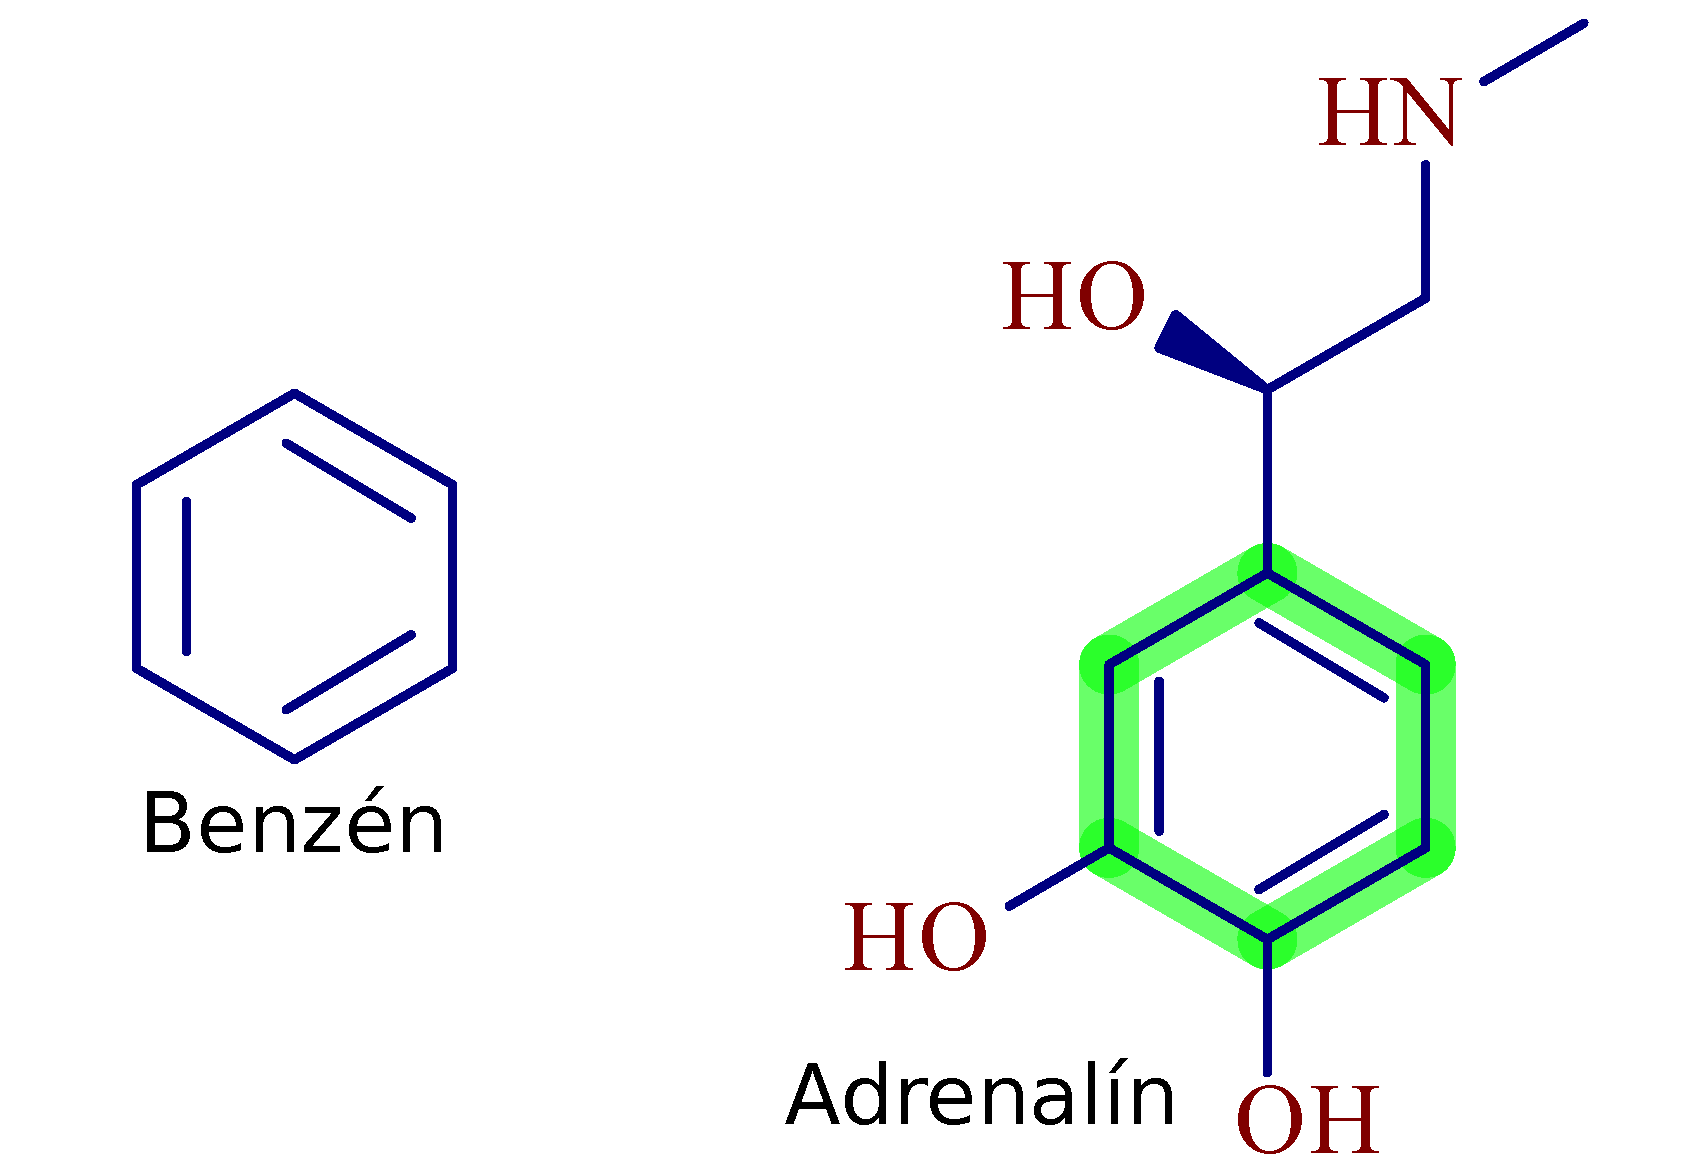
\includegraphics[height=9\baselineskip]{images/adrenaline.pdf}
	\caption{Vpravo: Chemická štruktúra adrenalínu obsahujúca atómy rôznych prvkov, aromatické väzby ako aj stereochémiu. Vľavo: Štruktúra benzénu. Zeleným je zvýraznený jeho výskyt v~adrenalíne ako podštruktúra.}
	\label{fig:adrenaline}
\end{figure}

Úlohou podštruktúrneho vyhľadávania je zistiť, či daná chemická štruktúra obsahuje zadaný vzor. Keďže sú chemické štruktúry reprezentované ako grafy, táto úloha odpovedá nájdeniu izomorfného podgrafu. Napriek tomu, že sa jedná o~NP-úplny problém, existujú algoritmy, ktoré ho umožňujú prakticky riešiť. Ullmann ako prvý navrhol takýto algoritmus \cite{ullmann}. Jeho princípom je prerezávanie stromu predstavujúceho pre\-hľa\-dá\-va\-ný priestor (obrázok \ref{fig:search_space_tree}) na základe splnenia určitej podmienky. Ak dôjde k~jej porušeniu, algoritmus už nemusí skúšať priradenie zvyšných vrcholov, čím výrazne redukuje počet porovnaní. 

\begin{figure}[!htb]
	\centering
	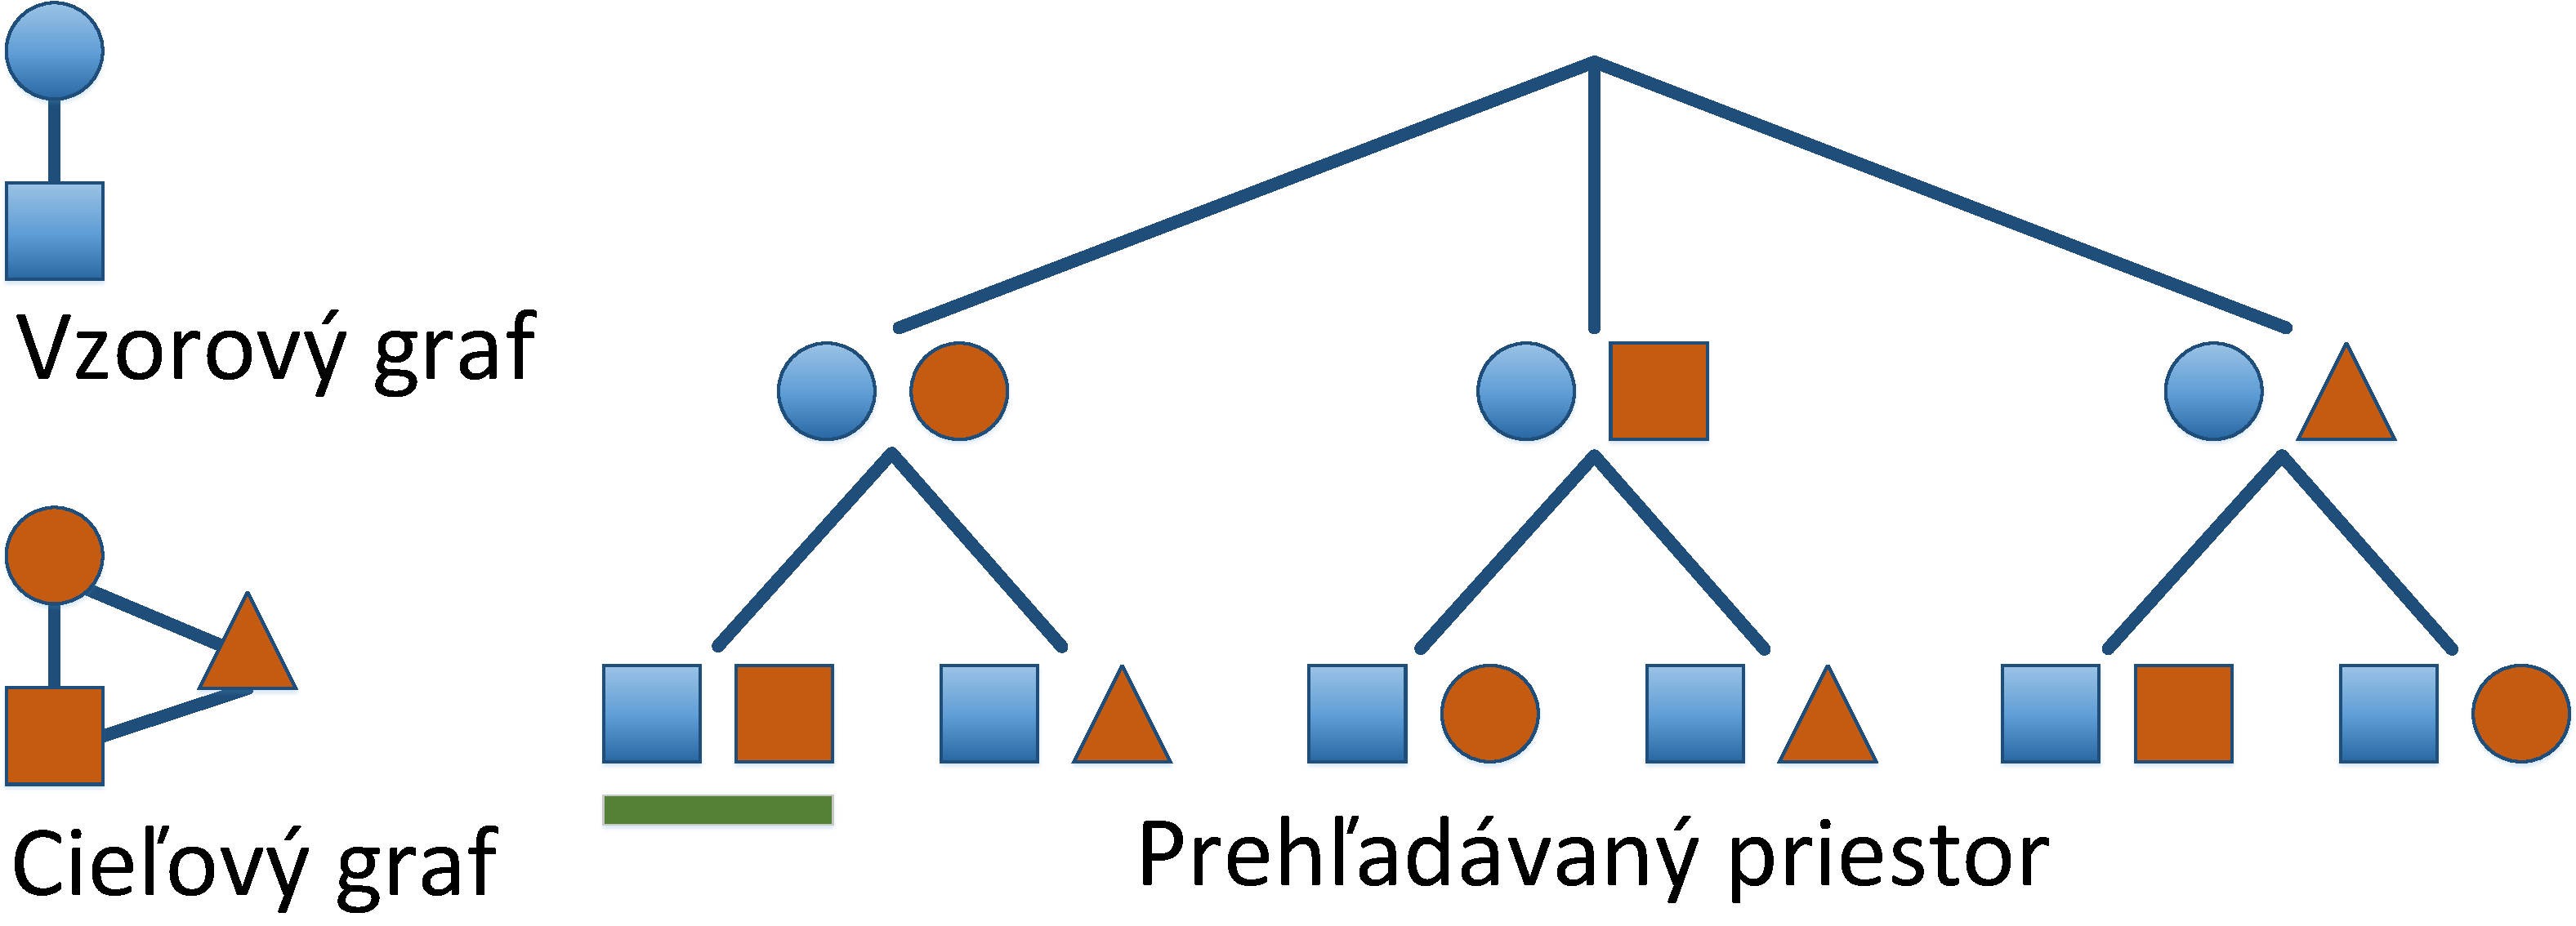
\includegraphics[width=1\linewidth]{images/ss_search_tree.pdf}
	\caption{Prehľadávaný priestor ako strom. Zelené podtrhnutie označuje vetvu, v~ktorej dôjde k~nájdeniu izomorfizmu. \cite{ri}}
	\label{fig:search_space_tree}
\end{figure}

Ullmannov algoritmus bol dlho jeden z~naj\-po\-uží\-va\-nej\-ších, ale medzi jeho nevýhody patrí hlavne vysoká pamäťová náročnosť. V~roku 1999 bol v~článku \cite{vf} predstavený algoritmus VF, a následne v~roku 2004 jeho vylepšená verzia VF2 \cite{vf2}, ktoré zlepšujú vlastnosti Ullmanovho algoritmu a riešia aj pamäťovú náročnosť. Tento algoritmus sa stal viac-menej štan\-dard\-nou implementáciou pre hľadanie izomorfných podgrafov v~chemických aplikáciách, a je možné ho nájsť použitý v~populárnych knižniciach ako sú RDKit alebo OpenBabel. Výskum však naďalej pokračoval a boli vyvinuté mnohé ďalšie algoritmy, ako napr. SND, LAD alebo FocusSearch. Zaujímavý je ale predovšetkým algoritmus RI predstavený v~roku 2011, ktorý je podľa meraní v~kontexte biochemických aplikácií lepší než všetky uvedené algoritmy \cite{ri}. Jeho princípom je zostavenie vyhľadávacej stratégie na zá\-kla\-de vzorového grafu v~kombinácii s~jednoduchými a rýchlymi obmedzujúcimi podmienkami. Rozhodli sme sa preto porovnať algoritmus RI so zaužívaným VF2 priamo pri probléme vyhľadávania v~databázach chemických látok.

\section{Molekulárne odtlačky}
Aj rýchlemu algoritmu pre hľadanie izomorfného podgrafu by trvalo veľmi dlhú dobu porovnať všetky zá\-zna\-my v~databáze. Ak budeme uvažovať, že by jedna inštancia problému trvala priemerne \SI{10}{\micro\second}, pre jeden dotaz v~databáze o~veľkosti 10 miliónov záznamov by iba samotný beh algoritmu v~najlepšom prípade spotreboval 100 sekúnd výpočetného času. S~narastajúcou databázou by potom tento čas ďalej lineárne narastal. Riešením tohto problému je použitie molekulárnych odtlačkov. Často sa jedná o~bitové polia, kde na jednotlivých bitoch sú zakódované rôzne dôležité topologické vlastnosti molekúl. Existuje mnoho druhov odtlačkov, no len niektoré z~nich sú vhodné pre pod\-štruk\-túrne vyhľadávanie. Jeden z~najrozšírenejších typov odtlačkov popísala firma Daylight. Jeho podstatou bolo kódovanie ciest v~grafe postupne narastajúcej dĺžky do odtlačku \cite{daylight_fp}. Keďže sa ale jedná o~komerčný produkt, jeho implementácia nebola voľne dostupná. Mnohé knižnice si preto vytvorili vlastné odtlačky tohto typu. Odtlačok pre podštruktúrne vyhľadávanie v~knižnici RDKit, \texttt{PatternFingerprint}, pracuje na podobnom prin\-cípe, ktorý zachytáva obrázok \ref{fig:fp}. Ako prvé sa vytvorí odtlačok, čiže bitové pole požadovanej dĺžky a všetky bity sa inicializujú na hodnotu 0. Pomocou algoritmu sa nájdu všetky výskyty niekoľkých preddefinovaných vzorov, ktoré značia významné topológie. Následne sa každý výskyt spolu s~vlastnosťami atómov a väzieb zahašuje na 32-bitové číslo, ktoré sa použije pre inicializáciu pseudonáhodného generátora čísel. Ten následne vygeneruje určený počet čísel, ktoré po modulu s~dĺžkou odtlačku slúžia ako indexy do bitového pola a do bitov na týchto pozíciach sa zapíše hodnota 1.

\begin{figure}[!htb]
	\centering
	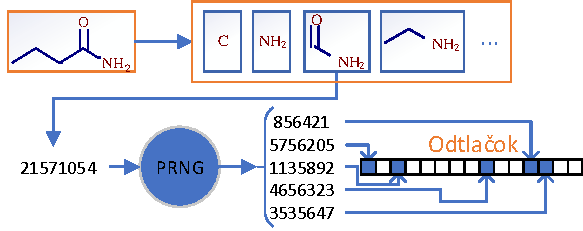
\includegraphics[width=1\linewidth]{images/daylight.pdf}
	\caption{Princíp vytvárania podštruktúrneho odtlačku v~knižnici RDKit. Preddefinované vzory sa vyhľadajú v~štruktúre a každý výskyt sa zahašuje na 32-bitové číslo, ktoré inicializuje PRNG. Ten vy\-ge\-ne\-ru\-je určený počet čísel slúžiacich ako indexy do bitového poľa, kde dôjde k~zmene hodnoty bitu.}
	\label{fig:fp}
\end{figure}

Samotný princíp použitia odtlačkov je pomerne priamočiary. Pre vzor sa určí odtlačok a následne sa porovnáva s~tými uloženými v~databáze. Iba ak všetky bity s~hodnotou 1 v~odtlačku vzoru sú nastavené na 1 aj v~odtlačku chemickej štruktúry, má zmysel použiť algoritmus pre vyhľadanie vzoru. V~opačnom prípade sa vzor v~štruktúre určite nenachádza. Takto je možné z~veľkej databázy získať pomerne malú množinu kandidátov, a tým výrazne obmedziť počet spustení algoritmu pre vyhľadanie podgrafu.

Presnosť odtlačku z~knižnice RDKit je približne 60\si{\percent}, čo znamená, že 40\si{\percent} kandidátov neobsahuje hľadaný vzor \cite{substruct_acc}. Ak by však databáza mala desať mi\-li\-ó\-nov záznamov a počet skutočných výsledkov by bol rádovo v~jednotkách tisícov, použitie odtlačku by zredukovalo počet prehľadávaných štruktúr o~viac ako 99\si{\percent}. V~takom prípade by aj pomerne zlý odtlačok s~presnosťou iba 5\si{\percent} dokázal výrazne zmenšiť prehľadávanú množinu.

\begin{figure*}[!htb]
	\centering
	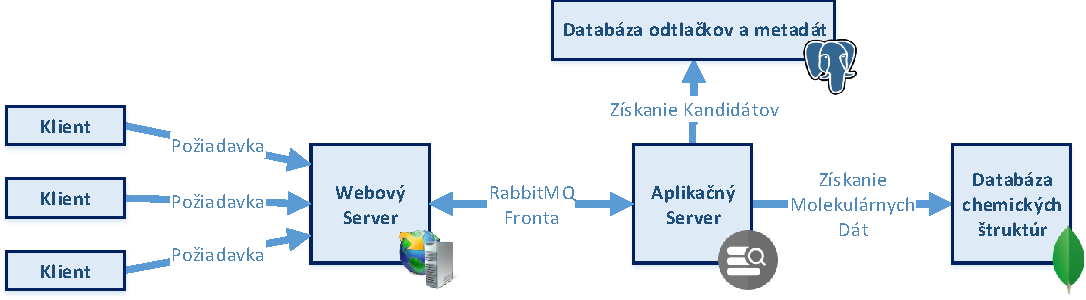
\includegraphics[width=1\linewidth]{images/system.pdf}
	\caption{Architektúra systému. Webový server prijíma požiadavky na vyhľadávanie od klientov a plní nimi RabbitMQ frontu. Aplikačný server vyberie požiadavku z~fronty a začne s~jej spracovaním. V~prvom kroku získa pomocou odtlačkov množinu kandidátov z~PostgreSQL databáze. Následne týchto kandidátov, pokiaľ nie sú v~pamäti, načíta z~MongoDB databáze chemických štruktúr. Pomocou algoritmu pre hľadanie izomorfného podgrafu skontroluje výskyt vzoru v~kandidátoch a výslednú množinu uloží k~požiadavke. Pri nasledovnom dotazovaní klienta na výsledok operácie je mu táto množina predaná.}
	\label{fig:system}
\end{figure*}

\section{Spôsob uloženia molekúl}
\label{sec:storage}
Chemické látky sú naprieč chemoinformatickými sy\-sté\-mami zdieľané najčastejšie pomocou textového for\-má\-tu MDL. Ten najskôr popisuje vlastnosti každého atómu a následne jednotlivé väzby ako indexy koncových atómov spolu s~vlastnosťami väzby \cite{mdl}. Viacero molekúl v~tomto formáte je potom možné zoskupiť do jedného súboru SDF. Jeho následnou kompresiou, napríklad metódou DEFLATE, je možné dosiahnuť uspokojivej veľkosti jedného záznamu. 

K~molekulám je však nutné v~procese vyhľadávania rýchlo pristupovať. Dátové štruktúry reprezentujúce molekuly naprieč systémom sú pamäťovo náročné, pretože bývajú optimalizované na rýchlosť a jednoduchosť použitia. Udržiavať takúto reprezentáciu v~pamäti pre všetky záznamy by kládlo príliš veľké nároky na jej veľkosť. Je preto zrejmé, že bude nutné molekuly komprimovať, a až v~prípade potreby vytvoriť odpovedajúcu dátovú štruktúru. Uvedený formát pre zdieľanie molekúl nie je na tieto účely vhodný, pretože jeho textová reprezentácia vyžaduje parsovanie textových reťazcov. Lepším riešením je serializovať dáta do binárneho formátu, akým je napríklad MessagePack. V~prostredí .Net existuje pre tento účel knižnica MessagePack-CSharp\footnote{\url{https://github.com/neuecc/MessagePack-CSharp}}, ktorá navyše podporuje následnú kompresiu algoritmom LZ4. 

Okrem voľby formátu je tiež nutné uvažovať, akým spôsobom dáta serializovať, aby doba spätného zí\-ska\-nia plnej reprezentácie ako aj veľkosť po serializácii boli čo najmenšie. Z~tohto dôvodu bolo vyskúšaných niekoľko rôznych prístupov, ktoré je možné nájsť v~repozitári odkazovanom v~abstrakte práce. Vyhodnotenie spolu s~porovnaním s~komprimovaným formátom SDF je možné nájsť v~sekcii \ref{sec:Results}.

Aj keď sa vďaka kompresii výrazne znížia pamä\-ťové nároky, pri priemernej veľkosti \SI{500}{\byte} na záznam by systémy s~databázami dosahujúcimi sto miliónov zá\-zna\-mov museli mať desiatky gigabajtov dostupnej pamäte iba na uloženie molekúl. Je preto nutné u\-va\-žo\-vať s~možnosťou, že nie všetky záznamy budú vždy v~pamäti. V~tom prípade je potrebné mať čo najrýchlejší spôsob prístupu k~nim. V~práci bolo vykonané porovnanie uloženia záznamov priamo v~sú\-bo\-ro\-vom systéme, kde každý súbor odpovedal jednej molekule, a v~NoSQL databáze MongoDB, kde sú molekuly uložené ako samostatné dokumenty.

\section{Celkový návrh systému}
Systém sa celkovo skladá zo štyroch častí, ktoré je možné vidieť na obrázku \ref{fig:system}. Webový server sprístupňuje systém užívateľom vo forme webových stránok a poskytuje API, cez ktoré klient spúšťa vyhľadávanie a dotazuje sa na jeho výsledok. Aplikačný server je zodpovedný za samotné vyhľadávanie v~databáze. Pre požadovaný vzor získa množinu kandidátov, v~ktorej následne skontroluje výskyt vzoru pomocou algoritmu pre hľadanie izomorfného podgrafu. Odtlačky a metadáta o~chemických látkach sú uložené v~PostgreSQL databáze. Tá je zodpovedná aj za určenie množiny kandidátov, ktorú vráti ako zoznam identifikátorov štruktúr. K~tomu bolo potrebné implementovať zásuvný modul, ktorý podporuje operáciu porovnania odtlačkov. V~prípade, že sa potrebné chemické štruktúry nenachádzajú na aplikačnom serveri, sú získané z~MongoDB databáze. Tá obsahuje iba samotné štruktúrne dáta.

Rozdelenie na dva databázové systémy má svoje opodstatnenie. PostgreSQL databáza umožňuje vytvorenie zásuvného modulu, v~ktorom sú vstavané funkcie implementované v~jazyku C a skompilované do dynamickej knižnice. Takáto funkcia je výrazne rýchlejšia, než odpovedajúca implementácia v~SQL. MongoDB vstavané funkcie nepodporuje, preto by nebolo možné určiť kandidátov priamo v~databáze, čo by vyžadovalo prenos všetkých odtlačkov na aplikačný server. Na druhú stranu ak je úlohou databázy iba nájsť určité kľúče a vrátiť asociované polia bajtov, ako je to v~prípade databázy chemických štruktúr, javí sa použitie nerelačnej databázy ako lepšie riešenie. V~prípade MongoDB je jednoduchšie aj horizontálne škálovanie, čiže pridávanie ďalších databázových serverov za účelom zvýšenia priepustnosti.

Webový a aplikačný server spolu komunikujú pomocou RabbitMQ fronty. RabbitMQ je open-source riešenie pre sprostredkovanie správ. Po prijatí po\-žia\-dav\-ky od klienta vytvorí webový server požiadavku na aplikačný server, v~ktorej uvedie parametre vy\-hľa\-dá\-va\-nia, a vloží ju do fronty. Aplikačný server sa pri spustení prihlási k~odberu týchto správ a zaviaže sa odpovedať. Po prijatí požiadavky spustí vyhľadávanie a vráti identifikátor operácie, ktorý je predaný klientovi. Ten ho použije pre následné dotazovanie sa na výsledok operácie. Toto riešenie umožňuje jednoducho pridávať do systému ďalšie aplikačné servery. Vo východzom nastavení budú požiadavky vo fronte rovnomerne rozdelené medzi dostupné aplikačné servery.

Nevýhodou rozdelenia systému je, že jednotlivé časti musia medzi sebou navzájom komunikovať, čo pridáva určitú réžiu. Taktiež správa takéhoto systému je náročnejšia. Na druhú stranu tento prístup umožňuje efektívnejšie škálovanie, kedy napríklad nie je nutné replikovať celú databázu, ak je potrebné zvýšiť priepustnosť v~algoritmickej časti.  


\section{Výsledky meraní}
\label{sec:Results}
Všetky nasledujúce merania boli vykonané na počítači s~touto špecifikáciou:
\begin{itemize}
	\item CPU -- AMD Ryzen 5 1600
	\item RAM -- 8GB, DDR4, 2933Mhz
	\item HDD -- WD5000AAKS, 500GB, 7200 otáčok/s
	\item SSD -- Samsung 850 EVO, 500GB
\end{itemize}
Prvým meraním bolo porovnanie dvoch algoritmov pre hľadanie izomorfného podgrafu a ich variánt. Konkré\-tne sa jednalo o~algoritmy VF2, VF2 s~radením, RI a teoretický algoritmus Best, ktorý pre konkrétnu dvojicu vždy zvolí najrýchlejší algoritmus spomedzi dostupných. Radenie pri VF2 spočíva v~zoradení pre\-hľa\-dá\-va\-ný\-ch vrcholov podľa protónového čísla prvku a stupňa vrcholu. Menej bežné prvky s~veľkým počtom susedov sa tak navštívia ako prvé. Meranie bolo vykonané nad reálnou databázou naplnenou miliónom chemických látok získaných z~databáze PubChem. Ako vzory bolo použitých tisíc najčastejších podštruktúr z~rovnakej databáze. Tie predstavujú najhorší možný prípad pri vyhľadávaní, pretože budú nájdené vo veľ\-kom množstve záznamov. Zoznam týchto podštruktúr bol získaný z~článku \cite{mol_cloud}. Aby merania odpovedali reálnemu prípadu užitia, algoritmus bol spustený iba pre záznamy, ktoré prešli testom odtlačkov. Pre každú dvojicu grafov bolo meranie zopakované päťkrát a z~nameraných časov bol zvolený medián, aby prípadné vyťaženie procesora iným procesom nemalo na meranie vplyv. Priemerná hodnota by v~prípade namerania výnimočne dlhého času bola skreslená. Následne bola pre každý algoritmus vypočítaná priemerná doba behu a počet prípadov, kedy bol daný algoritmus najrýchlejší spomedzi všet\-kých. Celkový počet inštancií bol\\$6472522$ a vzor sa našiel v $821939$ prípadoch. Výsledky sú uvedené v tabuľke \ref{tab:algo_meas}. Obrázok \ref{fig:algo_graph} zobrazuje namerané časy formou kumulatívneho histogramu. Ako je možné vidieť, algoritmus RI je najrýchlejší a za teoretickým algoritmom zaostáva iba o necelých \SI{5}{\percent}.

\begin{table}[h]
	\vskip6pt
	\caption{Porovnanie algoritmov pre hľadanie izomorfného podgrafu. Doba behu je priemerná hodnota pre jednu inštanciu a stĺpec najrýchlejší uvádza, koľko inštancií vyriešil daný algoritmus v~najkratšom čase.}
	\centering
	\begin{tabular}{l|r|r}
		\toprule
		Algoritmus & Doba behu (\si{\micro \second}) & Najrýchlejší (\#)\\
		\midrule
		VF2 & $37.014$ & $734941$ \\
		VF2 s~radením & $29.088$ & $96473$ \\
		RI & $12.817$ & $5641108$ \\
		Best & $12.259$ & \\
		\bottomrule
	\end{tabular}
	\label{tab:algo_meas}
\end{table}

\begin{figure}[!htb]
	\centering
	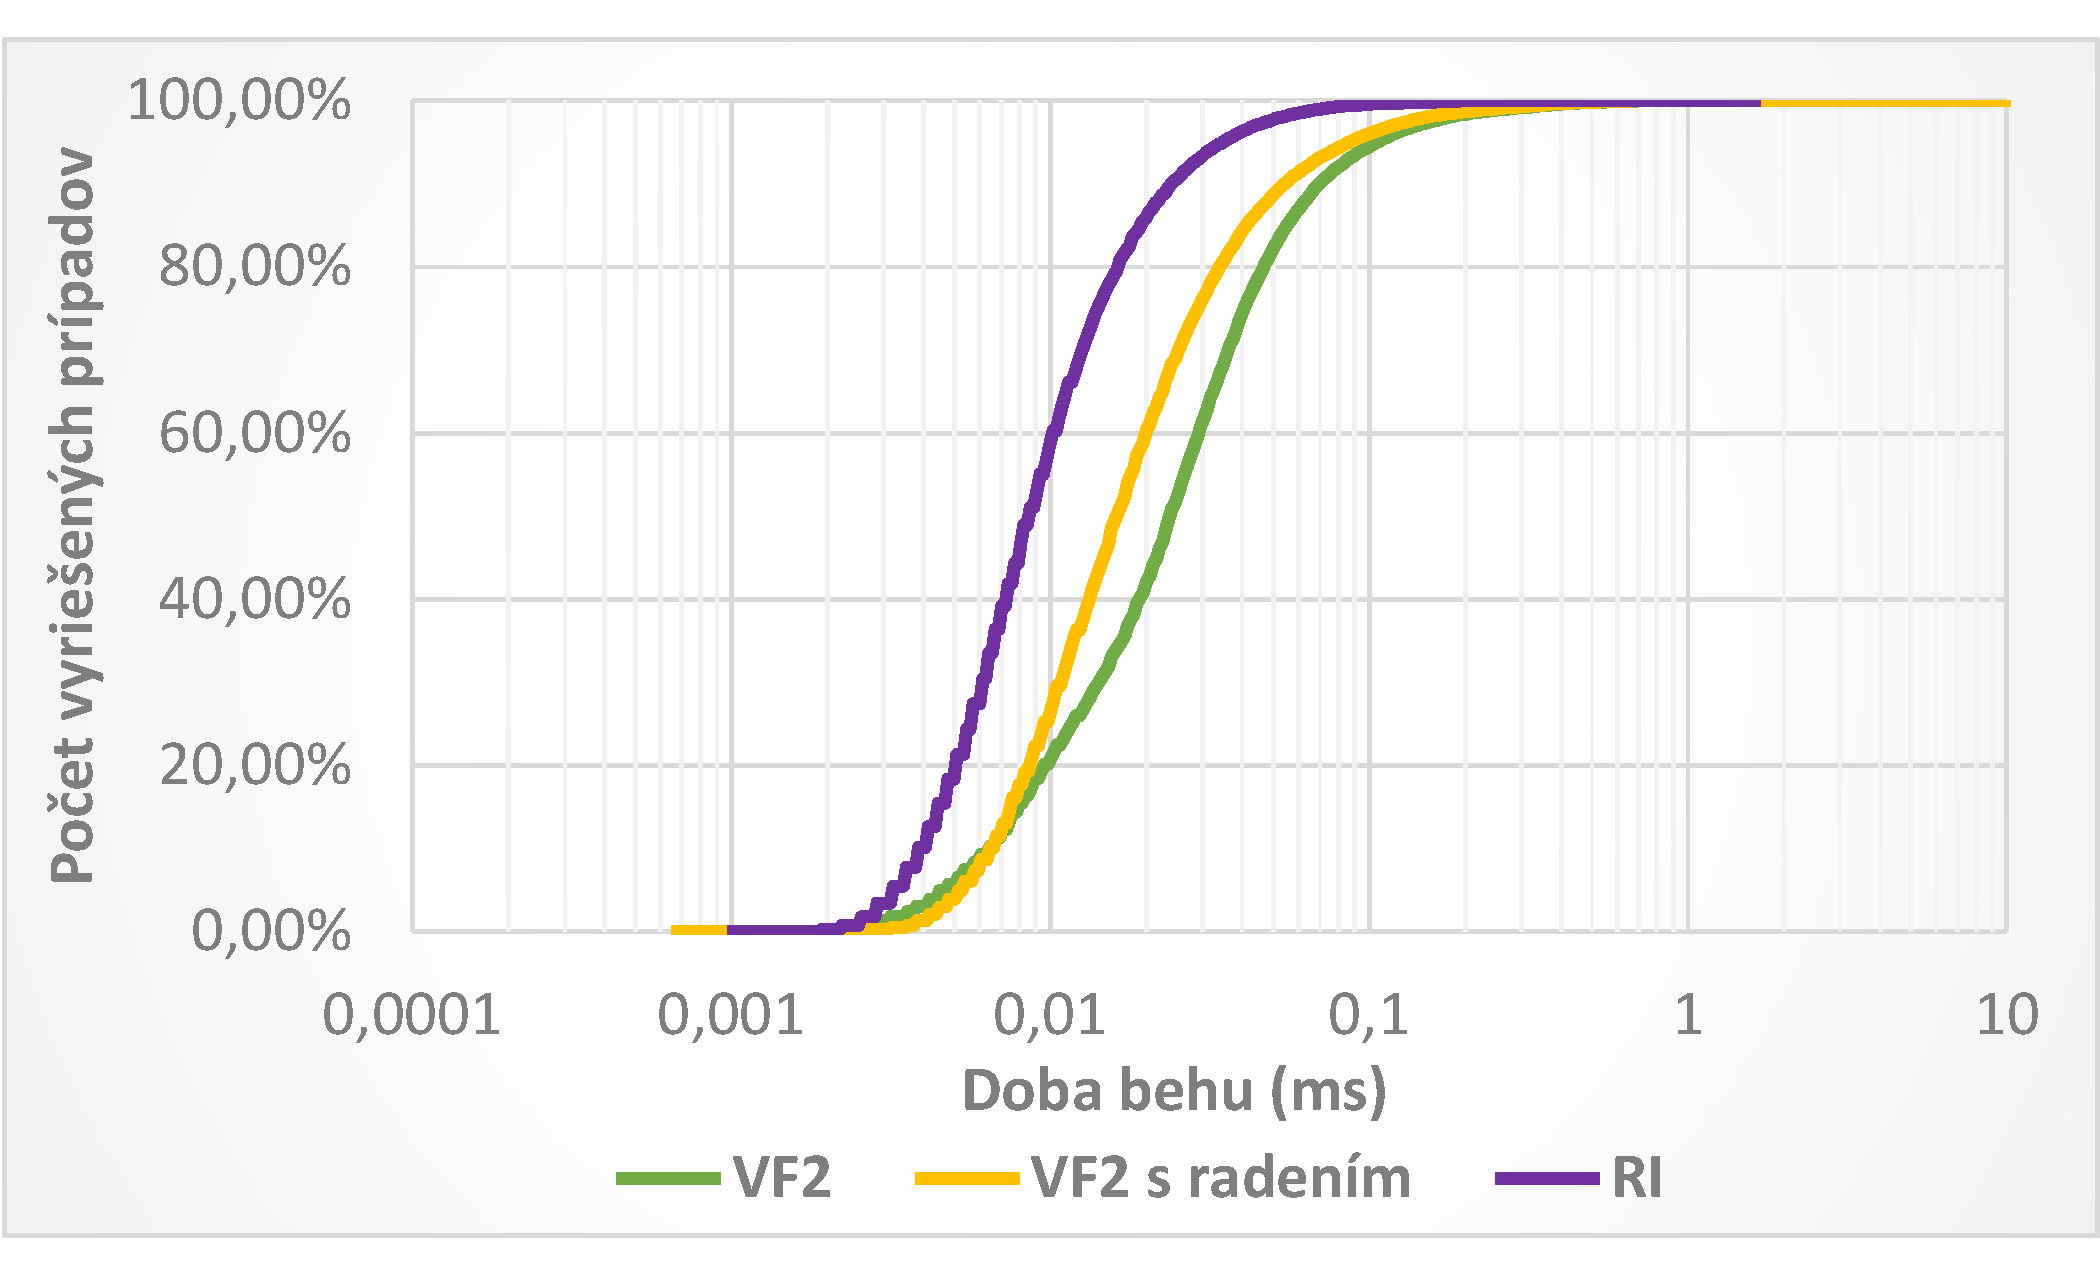
\includegraphics[width=1\linewidth]{images/algo_graph.pdf}
	\caption{Porovnanie algoritmov pre hľadanie i\-zo\-morf\-né\-ho podgrafu formou kumulatívneho hi\-sto\-gra\-mu. Interpretovať ho je možné ako počet inštancií, pre ktoré doba behu neprekračuje určitý čas. Napríklad v~prípade RI neprekračuje doba behu \SI{10}{\micro \second} v~\SI{60}{\percent} všetkých inštancií. }
	\label{fig:algo_graph}
\end{figure}

Ďalej bolo potrebné vykonať porovnanie jednotlivých formátov pre uloženie štruktúrnych dát predstavených v~časti \ref{sec:storage}. Sledovanými parametrami boli výsledná veľkosť v~bajtoch a rýchlosť opätovného získania plnej dátovej štruktúry. Formát MPM je za\-lo\-že\-ný na spomínanom serializačnom formáte MessagePack s~využitím LZ4 kompresie. Rozdiel medzi jednotlivými verziami je iba v~spôsobe uloženia vlastností atómov, preto väzby neboli súčasťou formátu pri tomto porovnaní. Meranie bolo vykonané na $100000$ náhodných molekulách z~databáze PubChem a desaťkrát zopakované. Spriemerované vý\-sledky je možné nájsť v~tabuľke \ref{tab:mpms}. Ako najoptimálnejšia verzia formátu sa javí MPM 3, kedy sú súradnice a prvky uložené v~poliach spoločných pre celú štruktúru a menej bežné vlastnosti atómov, ako napr. izotopy, sú uložené vo forme riedkych polí, kde každý prvok obsahuje index atómu a hodnotu danej vlastnosti.

\begin{table}[h]
	\vskip6pt
	\caption{Porovnanie viacerých spôsobov serializácie údajov o~atómoch v~chemických štruktúrach.}
	\centering
	\begin{tabular}{l|r|r}
		\toprule
		Formát & Veľkosť (\si{\byte}) & Deserializácia (\si{\micro\second}) \\
		\midrule
		MPM 1 & $553.167$ & $12.73$ \\
		MPM 2 & $540.187$ & $10.411$ \\
		MPM 3 & $400.58$ & $8.63$ \\
		MPM 4 & $519.614$ & $7.91$ \\
		\bottomrule
	\end{tabular}
	\label{tab:mpms}
\end{table}

Po pridaní informácií o~väzbách bolo možné formát MPM porovnať s~formátom SDF komprimovaným pomocou metódy DEFLATE. Aby bolo porovnanie spravodlivejšie, bol dátový typ pre súradnice vo formáte MPM zmenený z~\texttt{double} na \texttt{int}, keďže SDF podporuje pre súradnice iba hodnoty s~pevnou desatinnou čiarkou, ktorých rozsah sa zmestí do \texttt{int}. Porovnanie je možné nájsť v~tabuľke \ref{tab:sdfvsmpm}. Meranie bolo vykonané na $5000$ náhodných molekulách a výsledky sú spriemerované z~desiatich opakovaní. Výsledný formát má oproti komprimovanému SDF o~\SI{27}{\percent} menšiu veľkosť a umožňuje až trojnásobne rýchlejšiu deserializáciu do potrebnej dátovej štruktúry.

\begin{table}[h]
	\vskip6pt
	\caption{Porovnanie formátov MPM a SDF. Formáty, u ktorých nebol meraný čas deserializácie, sú uvedené iba pre porovnanie veľkosti, ich použitie by vzhľadom na existenciu lepšej varianty nedávalo zmysel.}
	\centering
	\begin{tabular}{l|r|r}
		\toprule
		Formát & Veľkosť (\si{\byte}) & Deserializácia (\si{\micro\second}) \\
		\midrule
		SDF & $4431.555$ & Nemerané \\
		SDF (DEFLATE) & $636.61$ & $259.283$ \\
		MPM (\texttt{double}) & $614.941$ & Nemerané \\
		MPM (\texttt{int}) & $465$ & $64.91$ \\
		\bottomrule
	\end{tabular}
	\label{tab:sdfvsmpm}
\end{table}

Ďalšie meranie malo za úlohu rozhodnúť, aký spô\-sob uloženia chemických štruktúr zvoliť. Prvá možnosť bolo uloženie priamo do súborového systému NTFS, preto bolo potrebné zmerať, či a ako sa mení prístupová doba k~súborom v~závislosti na počte súborov v~zložke. Okrem jednoduchých zložiek bola meraná prístupová doba aj v~stromovej štruktúre s~dvomi úrovňami, kde každá zložka obsahovala ďalších sto zložiek alebo súborov. Merania boli vykonané pre platňový disk aj SSD. Otvorených bolo 50 náhodných súborov v~zložke a meranie zopakované stokrát. Výsledná doba v~tabuľke \ref{tab:disk_access} je priemerom všetkých meraní. Na základe výsledkov je možné povedať, že optimálny počet sú\-bo\-rov v~zložke sa pohybuje okolo $1000$. Platňový disk u\-mož\-ňu\-je aj väčšie zložky, ale nad $10000$ súborov prístupová doba drasticky narastá. V~prípade SSD disku je tento nárast pozvoľnejší. Vytvorenie stromovej štruktúry nemalo na prístupovú dobu žiadny vplyv, preto je možné túto stratégiu využiť na zvyšovanie kapacity úložiska. 

\begin{table}[h]
	\vskip6pt
	\caption{Prístupová doba v~\si{\micro\second} k~súboru v~závislosti na počte súborov v~zložke pre súborový systém NTFS.}
	\centering
	\begin{tabular}{l|c|c|c|c}
		\toprule
		Počet & $100$ & $500$ & $1000$ & $5000$ \\
		\midrule
		HDD & $97.478$ & $103.041$ & $106.291$ & $117.142$ \\
		SSD & $102.626$ & $113.461$ & $129.938$ & $175.376$ \\
		\midrule[2px]
		Počet & $10000$ & $100000$ & $300000$ & Strom (100)\\
		\midrule
		HDD & $120.725$ & $1059.978$ & $3485.66$ & $96.07$
		 \\
		SSD & $214.802$ & $455.916$ & $529.47$ & $110.796$ \\
		\bottomrule
	\end{tabular}
	\label{tab:disk_access}
\end{table}

\begin{table}[h]
	\vskip6pt
	\caption{Priemerná doba získania serializovaných dát che\-mic\-kej štruktúry z~úložiska. Metóda \texttt{ReadAllBytes} číta obsah súborov v~stromovej štru\-ktú\-re. Metóda \texttt{Find} získava dáta z~databáze MongoDB, kde číslo uvádza počet súbežne zí\-ska\-ný\-ch záznamov. }
	\centering
	\begin{tabular}{l|c}
		\toprule
		Metóda & Doba získania dát (\si{\micro\second})  \\
		\midrule
		\texttt{ReadAllBytes} & $211.936$ \\
		\texttt{Find} 1       & $234.376$ \\
		\texttt{Find} 10      & $35.108$ \\
		\texttt{Find} 100     & $13.408$ \\
		\texttt{Find} 1000    & $12.137$ \\
		\bottomrule
	\end{tabular}
	\label{tab:storage_benchmark}
\end{table}

Po určení vhodnej veľkosti zložiek bolo možné vytvoriť úložisko v~súborovom systéme a porovnať ho s~databázou MongoDB. V~súborovom systéme na SSD disku bola vytvorená dvoj-úrovňová stromová štruktúra, kde každá zložka obsahovala najviac $1000$ súborov. Každá chemická štruktúra bola uložená ako jeden súbor, ktorého obsah sa čítal v~prostredí .Net pomocou funkcie \texttt{File.ReadAllBytes}. V~databáze MongoDB uloženej taktiež na SSD disku bola vytvorená nová kolekcia záznamov, ku ktorej sa pristupovalo pomocou oficiálneho MongoDB ovládača pre .Net. K~získaniu požadovaných záznamov bola použitá funkcia \texttt{collection.Find}, ktorej bol ako parameter predaný filter so zoznamom identifikátorov požadovaný záznamov. Keďže tento spôsob narozdiel od súborového úložiska umožňuje získať viacero záznamov jedným príkazom, boli zmerané časy pre rôzny počet súbežne získaných záznamov. Do oboch dátových úložisiek bolo uložených milión chemických štruktúr s~priemernou veľkosťou \SI{524}{\byte} v~serializovanej reprezentácii. Následne sa merala doba získania serializovaných dát pre $10000$ náhodných chemických štruktúr, každé meranie bolo desaťkrát zopakované a výsledky spriemerované. V~tabuľke \ref{tab:storage_benchmark} je možné nájsť výslednú priemernú dobu načítania dát jednej chemickej štruktúry pre uvedené metódy.

Ako je možné vidieť vo výsledkoch, získanie dát pre jeden záznam v~databáze približne odpovedá zí\-ska\-niu dát zo súboru, avšak pri vyžiadaní viacerých záznamov z~databáze zároveň je databázové riešenie rádovo rý\-chlej\-šie. Zrýchlenie je najvýraznejšie medzi získaním jenoho a desiatich záznamov. S~ďalej sa zvyšujúcim počtom je postupne toto zrýchlenie menej výrazné, zatiaľ čo rastú pamäťové nároky na uloženie dát. Ako optimálna sa preto javí hodnota medzi $100$ až $1000$ súbežne získanými záznamami.

Po sčítaní doby získania štruktúrnych dát z databázy, ich deserializácie a priemernej doby behu algoritmu RI zistíme, že doba spracovania jedného kandidáta sa~pohybuje okolo \SI{91}{\micro\second}. Ceľková doba vy\-hľa\-dá\-va\-nia potom závisí od~počtu kandidátov, ktorých je nutné skontrolovať. V~prípade použitia odtlačku s~vysokou presnosťou bude ich počet závisieť predovšetkým od~veľ\-ko\-sti databáze a vstupného vzoru. V prípade zadania vzoru, ktorý je reálne možné nájsť ako podštruktúru v \SI{30}{\percent} databázových záznamov bude vyhľadávanie z~prin\-cí\-pu trvať veľmi dlhú dobu. Takéto obecné vzory ale ne\-bý\-va\-jú pre užívateľov príliš za\-u\-jí\-ma\-vé. Navyše aj v~prípade množiny najčastejších vzorov, spomenutej začiatkom tejto časti, bol v~\SI{80}{\percent} prípadov počet kandidátov menší ako \SI{1}{\percent} veľkosti databáze. Ak uvážime databázu s~10 miliónmi záznamov, \SI{1}{\percent} by predstavovalo sto tisíc kandidátov. Pre takúto kandidátnu mno\-ži\-nu by doba spracovania bola \SI{9.1}{\second} a tento čas by bolo možné ďalej skrátiť paralelným spracovaním vo~viacerých vláknach. Experimenty na~takto veľkých kandidátnych množinách potvrdili predpovedanú dobu vyhľadávania. 

%--------------------------------------------------------
%--------------------------------------------------------
%--------------------------------------------------------
%--------------------------------------------------------
\section{Záver}
\label{sec:Conclusions}

%\textbf{[Paper Summary]} What was the paper about, then? What the reader needs to remember about it?
%\phony{Lorem ipsum dolor sit amet, consectetur adipiscing elit. Proin vitae aliquet metus. Sed pharetra vehicula sem ut varius. Aliquam molestie nulla et mauris suscipit, ut commodo nunc mollis.}
V~tomto článku bol predstavený celkový návrh systému pre podštruktúrne vyhľadávanie v~databázach che\-mic\-kých látok. Taktiež sa článok zaoberal optimalizáciou jednotlivých častí a vyhodnotením viacerých alternatív.

%\textbf{[Highlights of Results]} Exact numbers. Remind the reader that the paper matters.
%\phony{Lorem ipsum dolor sit amet, consectetur adipiscing elit. Sed tempus fermentum ipsum at venenatis. Curabitur ultricies, mauris eu ullamcorper mattis, ligula purus dapibus mi, vel dapibus odio nulla et ex. Sed viverra cursus mattis. Suspendisse ornare semper condimentum. Interdum et malesuada fames ac ante ipsum.}
Algoritmus RI sa ukázal až trikrát rýchlejší oproti zaužívanému algoritmu VF2. V~súborovom systéme NTFS po prekročení 10000 súborov v~zložke narastá prístupová doba k~súboru lineárne s~počtom súborov. Riešením je vytvorenie stromových štruktúr pomocou adresárov. V~prípade dostatku pamäte RAM však umožňuje NoSQL databáza MongoDB až de\-sať\-ná\-sob\-ne rýchlejšie načítanie dát oproti uloženiu štruktúrnych dát do samostatných súborov v~súborovom systéme. 

%\textbf{[Paper Contributions]} What is the original contribution of this work? Two or three thoughts that one should definitely take home.
%\phony{Lorem ipsum dolor sit amet, consectetur adipiscing elit. Praesent posuere mattis ante at imperdiet. Cras id tincidunt purus. Aliquam erat volutpat. Morbi non gravida nisi, non iaculis tortor. Quisque at fringilla neque.}
Pri optimalizácii systému je nutné uvažovať o~kaž\-dej jeho časti v~súvislosti s~ostatnými. Použitie rý\-chlej\-šie\-ho algoritmu bude mať na zrýchlenie systému minimálny dopad, ak sa väčšinu času čaká na načítanie dát. Taktiež je dôležité vhodne rozdeliť úlohy. Na\-prí\-klad presunutie kontroly odtlačkov priamo do databáze v~konečnom dôsledku zníži jej zaťaženie, pretože sa za cenu výpočtu výrazne zmenší objem prenášaných dát. V~súvislosti s~tým je vhodné pripomenúť, že aj pomerne zlý topologický index s~nízkou presnosťou môže podstatne obmedziť spracovávanú množinu záznamov.

%\textbf{[Future Work]} How can other researchers / developers make use of the results of this work?  Do you have further plans with this work? Or anybody else?
%\phony{Lorem ipsum dolor sit amet, consectetur adipiscing elit. Suspendisse sollicitudin posuere massa, non convallis purus ultricies sit amet. Duis at nisl tincidunt, maximus risus a, aliquet massa. Vestibulum libero odio, condimentum ut ex non, eleifend.}
V~prípade návrhu podobného systému predstavuje voľba rôznych metód a technológii náročnú úlohu a často sa nezaobíde bez podrobných meraní. Problém riešený v~tejto práci je veľmi špecifický, no výsledky a koncepty sú relevantné pre aplikácie zaoberajúce sa hľadaním vzorov v~početných databázach grafov. 

\section*{Poďakovanie}
Rád by som poďakoval Ing. Zbyňkovi Křivkovi Ph.D za odborné vedenie práce a pomoc pri písaní tohto článku.

%--------------------------------------------------------
%--------------------------------------------------------
%--------------------------------------------------------
%	REFERENCE LIST
%--------------------------------------------------------
%--------------------------------------------------------
\phantomsection
\bibliographystyle{unsrt}
\bibliography{2018-ExcelFIT-SubStructure-bib}

%--------------------------------------------------------
%--------------------------------------------------------
%--------------------------------------------------------
\end{document}